% !TEX root = ../thesis_main.tex
\chapter{Introduction}

\section{What are Carbon Nanotubes?}

Carbon allotropes such as fullerenes, carbon nanotubes, and graphene have attracted substantial interest due their unique properties and their exemplary use as model systems for investigations of many-body physics in low-dimensional systems \cite{avouris2000carbon, dresselhaus2001introduction,jorio2007carbon, nanot2012optoelectronic, zaytseva2016carbon, soavi2016ultrafast}. In particular, carbon nanotubes (CNTs), being one-dimensional (1-D) materials, have shown great promise for applications in next-generation optoelectronic devices and have established a role as one of many leading candidate materials to replace other conventional semiconducting materials in such applications \cite{nanot2012optoelectronic}. Some of these applications include terahertz polarizers \cite{ren2009carbon}, transistors \cite{qiu2017scaling}, light-emitting devices \cite{liu2015electrically}, and solar cells \cite{kongkanand2007single}.

\begin{figure}[H]
	\centering
	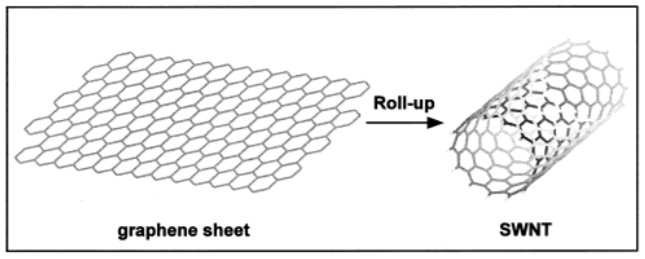
\includegraphics[scale=0.8]{images/chapter_intro/rolled_up_graphene.png}
	\caption{Schematic showing how a 2-D sheet of graphene is rolled to form a hollow nanotube. Reproduced and modified from Ref.\ \cite{odom2000structure}.}
\end{figure}

CNTs are best visualized as two-dimensional sheets of graphene that have been rolled up to form hollow, cylindrical structures \cite{odom2000structure,charlier2007electronic}. Their 1-D character arises due to their unusual aspect ratios as CNTs can have diameters of 1 $-$ 3 nanometers whilst possessing lengths on the order of hundereds of nanometers to micrometer length scales \cite{zaytseva2016carbon, ando1997excitons}. This essentially confines their electrons to move only in one direction and significantly enhances electron-electron interactions \cite{ando1997excitons}. Moreover, CNTs can behave as either metals or semiconductors depending on their crystal structure. Owing to such features, CNTs therefore manifest atypical, anisotropic optical and electronic properties \cite{dresselhaus2001introduction, jorio2007carbon, weismanKonoBook}.

\section{Ultrafast Spectroscopy of Carbon Nanotubes}

Ultrafast spectroscopy provides a means of investigating the microscopic phenomena associated with the macroscopic electronic and optical properties of many materials. This technique incorporates the use of ultrashort laser pulses as to resolve microscopic dynamics occuring on femtosecond timescales \cite{shah1996ultrafast}. It has been successfully used in many instances to study both coherent and noncoherent phenomena occuring in many systems. For instance, ultrafast methods have been employed in studies of carrier relaxation dynamics in bulk semiconductors \cite{beard2000transient, hendry2007exciton, pijpers2009assessment} and their nanostructures \cite{johar2019ultrafast, zhang1997ultrafast, hopper2018ultrafast}, coherent phonons \cite{farztdinov1997spectral, melnikov2018coherent} electronic properties of superconductors \cite{zhang2016stimulated, kaindl2005dynamics, mankowsky2014nonlinear}, spin dynamics of magnetic materials \cite{beaurepaire1996ultrafast, kirilyuk2010ultrafast, kim2016ultrafast}, as well as the optical Stark effect \cite{von1986optical, frohlich1985observation, sie2015valley}.

Transient absorption and time-resolved photoluminescence are two ultrafast spectroscopy techniques commonly employed in studies of CNTs. In effect, transient absorption measurements probe how the absorption associated with optical resonances change on a femtosecond timescale after photoexcitation induced by an ultrashort pump pulse \cite{shah1996ultrafast}. Time-resolved photoluminescence instead reveals how light emission, emerging from radiative recombination of electron-hole pairs, evolves on ultrafast timescales after such excitations \cite{shah1996ultrafast}. These two methods provide complementary perspectives of the optical properties of materials. Despite this, the interpretations of ultrafast spectroscopy data obtained for nanotubes has been partially obfuscated by the quality of samples studied.

\begin{figure}[ht]
	\centering
	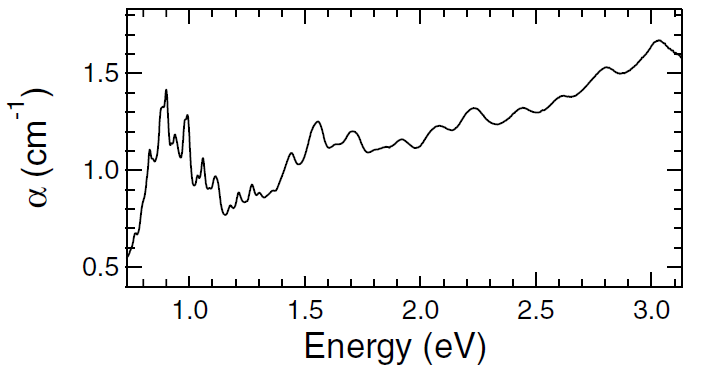
\includegraphics[scale=0.7]{images/chapter_intro/abs_gordana_modified}
	\caption{Optical absorption spectrum of a HiPco SWCNT dispersion. Each peak corresponds to an electronic transition of a particular CNT species. These emerge due to the optical responses of semiconducting and metallic nanotubes. Due to the close proximity of the resonances, each peak associated with one nanotube species has a tendency to spectrally overlap with resonances belonging to other types of nanotubes. This makes it hard to isolate the carrier dynamics associated with one particular species. Reproduced and modified from Ref.\ \cite{ostojic2004interband}.}
	\label{fig:abs_gordana_intro}
\end{figure}

Standard CNT growth processes create many different types of nanotubes, each with their own set of optical resonances \cite{prasek2011methods}. In the past, methods for creating samples enriched by only one species had not been well-established. As a result, many early studies used samples containing an ensemble of several different species of CNTs. One issue has been that optical responses of different nanotubes easily mix together, making it harder to distinguish between the dynamics associated with each individual species. As an example, Figure \ref{fig:abs_gordana_intro} shows the optical absorption spectrum of the sample used by Ostojic \textit{et al}.\ (2004) \cite{ostojic2004interband}. Here, the optical resonances spectrally overlap with other nearby resonances.

In ultrafast spectroscopy measurements, this means that photoexcitations in these ensembles will generate a combination of resonant and nonresonant excitations whose respective responses cannot always be individually resolved \cite{ostojic2004interband}. When optically pumping at a given photon energy, real carriers will be created in nanotubes with resonances below the pump photon energy. Apart from this, multiphoton processes will also create carriers in other nanotubes possessing band gap energies above the pump photon energy. In transient absorption measurements, at any given photon energy the optical probe will potentially detect carrier dynamics from all nanotubes within the ensemble. For photoluminescence measurements, emission peaks from different species will also spectrally overlap with other neighboring emission peaks.

These challenges pose significant barriers to the knowledge needed to incorporate CNTs in different technological domains. For optoelectronic applications such as lasers, we would want to understand different aspects of carrier relaxation in CNTs to establish whether favored conditions like population inversion can be easily achieved. Without the ability to isolate and investigate optical response of a single nanotube species at a time, it becomes difficult to distinguish between carrier relaxation processes associated with carrier-carrier scattering or carrier-phonon scattering. Furthermore, in the context of developing ultrafast all-optical switching devices, coherent processes need to be well understood. However, in CNT ensembles, nonresonant excitations can easily generate incoherent processes in other CNTs that are not of interest, thereby masking the presence of any coherent phenomena exhibited by the CNTs under investigation.

Fortunately, in light of these difficulties recent developments in sample preparation techniques have made high-purity, single-chirality samples more accessible \cite{komatsu2010comprehensive,liu2011large, janas2018towards, ichinose2017extraction, zheng2019sorting}. Figure \ref{fig:abs_fumiya} shows the absorption spectrum of a sample created using more up-to-date techniques. A large majority of the absorption peaks are easily recognized as optical transitions of (6,5) carbon nanotubes. Studying purer samples such as this will prove to be beneficial in future efforts to clarify outstanding questions regarding the optical properties of SWCNTs.

\begin{figure}
	\centering
	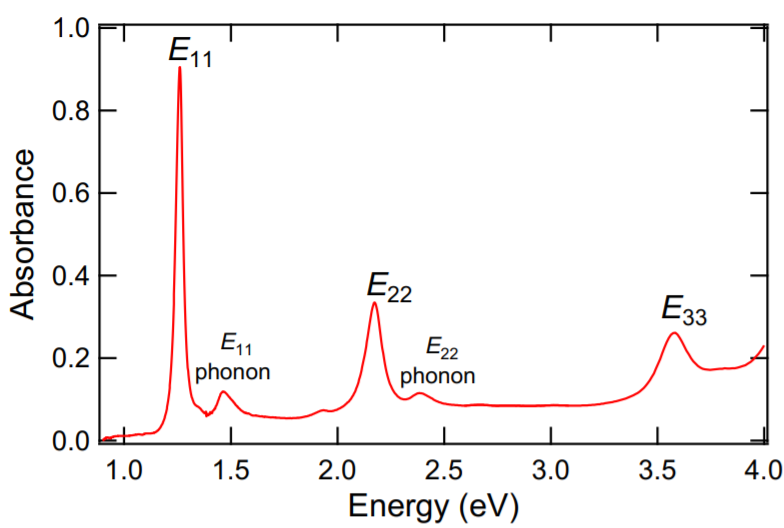
\includegraphics[scale=0.6]{images/chapter_intro/abs_fumiya}
	\caption{Absorption spectrum of a (6,5)-enriched SWCNT ensemble. The labeled peaks all correspond to optical transitions of (6,5) carbon nanotubes. Reproduced from Ref.\ \cite{katsutani2019direct}.}
	\label{fig:abs_fumiya}
\end{figure}

\section{Thesis Outline}

This thesis focuses on the use of ultrafast spectroscopy to investigate the carrier dynamics of high-purity, CNT samples. Chapter 2 provides a more thorough introduction to some of the basic properties of carbon nanotubes. Chapter 3 further explores prior ultrafast spectroscopy studies of carbon nanotubes. Chapter 4 illustrates the relevant experimental procedures used in this work. Chapters 5 and 6 present experimental results and discussion.  Chapter 5 focuses ultrafast coherent phenomena that occur within the pump pulse width, including the optical Stark effect and coherent pump-probe mixing.  These processes are observable when the pump photon energy is below the gap (creating virtual carriers) or resonant with the lowest-energy exciton state.  Chapter 6 describes incoherent carrier relaxation processes that occur when the pump photon energy is higher than the bandgap and thus the pump creates real carriers. The photocarriers rapidly decay through carrier-carrier scattering and carrier-phonon scattering, subsequently bleaching the exciton absorption peak.  Finally, in Chapter 7, we summarize the new findings made in this thesis work and provide our theoretical interpretations.  Furthermore, we discuss open questions and possible future studies.
